% !TeX encoding = UTF-8
% !TeX spellcheck = en_US
\documentclass[11pt, a4paper]{article}

% The title of the current document to be produced.
\newcommand{\doctitle}{Course Outline}
\newcommand{\labactivities}{\bluetext{\textbf{Lab:} activities covering discussed topics.}}
%
\setlength{\unitlength}{1in}
\renewcommand{\arraystretch}{2}

%------------------------------------------------------------
% Import commands for both teacher and course information.  | 
% NOTE: Change your teacher and course info in these files. |
%------>------>------>------>------>------>------>------>-->|
%% ==================================
%% ===== Teacher info             ===
%% ==================================
%%
\newcommand{\instructor}{Instructor Name}
\newcommand{\office}{Office number}
\newcommand{\hours}{By appointment}
\newcommand{\phone}{514.999.9999}
\newcommand{\college}{College Name}
\newcommand{\email}{username@mycollege.ca}
\newcommand{\faculty}{Faculty of Science and Technology}
\newcommand{\department}{Computer Science Technology}
                              %|
%% ==================================
%% ===== Course-specific commands ===
%% ==================================

%- Instructions: change course info here. 
\newcommand{\semester}{Winter 2022}

\newcommand{\csection}{00001 \& 00002}
\newcommand{\ponderation}{2-4-3 (Theory-Lab-Homework)}
\newcommand{\coursetitle}{Course Title}
\newcommand{\coursenumber}{[Course Number]}
\newcommand{\prerequisite}{All porgram courses semesters 1-4}
                               %|   
%
%------------------------------------------------------------
%-- Import packages and custom command definitons.          |
%------>------>------>------>------>------>------>------>-->|
% ftp://ftp.dante.de/tex-archive/fonts/bbding/bbding.pdf
%https://ctan.math.illinois.edu/fonts/bbding/bbding.pdf
\usepackage{fancyhdr, lastpage, bbding, pmboxdraw}
%\usepackage[usenames,dvipsnames]{color}
\PassOptionsToPackage{usenames,dvipsnames}{xcolor}

\usepackage{verbatim} % used to display code
\usepackage{fancyvrb}
\usepackage{acronym}
\usepackage{amsthm}
%\usepackage{listings}
\usepackage{caption}
%\usepackage{multirow}
\usepackage{xcolor}
\usepackage{enumitem}
\usepackage{tabularx}
\usepackage{sectsty}
% pifont package doc at: https://ctan.math.ca/tex-archive/macros/latex/required/psnfss/psnfss2e.pdf
% pifont is used to define custom list and style list items using the \ding command. 
\usepackage{pifont} 

% Select what to do with todonotes: 
% \usepackage[disable]{todonotes} % notes not showed
%\usepackage[draft]{todonotes}   % notes showed
%\usepackage[margin=1in]{geometry}
\usepackage[colorlinks,pagebackref,pdfusetitle,urlcolor=blue,citecolor=darkblue,linkcolor=blue,bookmarks,plainpages=false]{hyperref}
\usepackage{titlesec}  
\usepackage[open,openlevel=1]{bookmark}

%-- @see http://ctan.sharelatex.com/tex-archive/fonts/fontawesome/doc/fontawesome.pdf
% Font Awesome  http://ctan.math.washington.edu/tex-archive/fonts/fontawesome5/doc/fontawesome5.pdf
% https://muug.ca/mirror/ctan/fonts/fontawesome5/doc/fontawesome5.pdf
\usepackage{fontawesome5}
\usepackage{fontawesome}
%---------------------------------
% ==== Font setup.
%---------------------------------
%\usepackage{lmodern}
%\usepackage{mathptmx}
%\usepackage{times}
\usepackage{tgbonum}
\usepackage[utf8x]{inputenc}
\usepackage[T1]{fontenc}
%---------------------------------
\usepackage{booktabs}
 
% The margins at the bottom of the page has been reduced.
% this allows for a slim footer.
\usepackage[left=1in,right=1in,top=1in,bottom=0.7in]{geometry}

% Original size:
%\usepackage[inner=1.5cm,outer=1.5cm,top=1.5cm,bottom=.5cm,margin=1in]{geometry}
%\usepackage[margin=1in]{geometry}
\pagestyle{empty}
\usepackage{graphicx}
\usepackage{multicol}
\usepackage{blindtext}
                          %|  
%======================================
% Creates an underlined non-numbered section header.
%\setcounter{secnumdepth}{0}
\makeatletter
\renewcommand\@seccntformat[1]{}
\makeatother

%----------------------------------------------------------------
%--> \customsection: makes unumbered small caps section heading.|
%----------------------------------------------------------------
\titleformat*{\section}{\bfseries\large\scshape}
\newcommand{\customsection}[1]{
	\section{\textsc{#1}}\label{sec:#1} 
	% Reduce the vertical space below section headings.
	\vspace{-0.1cm} 
}
%--------------------------------------------------------
%--> \customhrule: makes a customized rule whose width  | 
%                  should be passed as parameter.       |
%--------------------------------------------------------
\newcommand{\customhrule}[1]{
	\rule[1.4pt]{\linewidth}{#1}
}
%------------------------------------------------------
%--> \doublerule: makes a double rule.                |
%------------------------------------------------------ 
\newcommand{\doublerule}[1][.4pt]{
	\noindent
	\makebox[0pt][l]{\rule[.7ex]{\linewidth}{#1}}%
	\rule[1pt]{\linewidth}{#1}\par} 
%===== Custom Ruler commands  ==================
\renewcommand{\headrulewidth}{1pt}
\renewcommand{\footrulewidth}{0.4pt}
% Disable spaces between list items in a labeled list.
\setlist{noitemsep}
 
%-------------------------------------------------------------
%= The followig are declaraions of custom Lists              =
%-------------------------------------------------------------
%
%======= Green rectangles list =======================
% \Rectangle from bbind
\newlist{greenrectangles}{itemize}{4}
%\setlist[greenrectangles]{topsep=4pt,partopsep=0pt,itemsep=3pt,parsep=0pt,labelindent=0.5cm,leftmargin=*}
\setlist[greenrectangles]{itemsep=5pt,parsep=0pt,topsep=4pt,partopsep=3pt}
\setlist[greenrectangles,1]{font=\color{darkred},label={\color{darkgreen}{\Rectangle}}}

%======= Alphabetical  list =======================
\newlist{alphalist}{enumerate}{9}
\setlist[alphalist]{topsep=4pt,partopsep=0pt,itemsep=3pt,parsep=0pt,labelindent=0.5cm,leftmargin=*}
\setlist[alphalist,1]{label=\textbf{\alph*)}}
%======= Non-numbered list =======================
\newlist{itemizedlist}{itemize}{9}
\setlist[itemizedlist]{topsep=4pt,partopsep=0pt,itemsep=3pt,parsep=0pt,labelindent=0.5cm,leftmargin=*}
%\setlist[itemizedlist,1 ]{label=\textbf{\alph*)}}

%======= Arrowed list =======================
\newlist{arrows}{itemize}{4}
\setlist[arrows]{topsep=4pt,partopsep=0pt,itemsep=3pt,parsep=0pt,labelindent=0.5cm,leftmargin=*}
\setlist[arrows,1]{font=\color{darkred},label={\HandRight}}

%======= Bordered square list =======================
% Colorize the selected symbol? 
% ❏
\newlist{borderedsquare}{itemize}{4}
\setlist[borderedsquare]{topsep=4pt,partopsep=0pt,itemsep=3pt,parsep=0pt,labelindent=0.5cm,leftmargin=*}
\setlist[borderedsquare,1]{label=\ding{111}}

%======= Filled, curved arrow list =======================
\newlist{curveddarrow}{itemize}{4}
\setlist[curveddarrow]{topsep=4pt,partopsep=0pt,itemsep=3pt,parsep=0pt,labelindent=0.5cm,leftmargin=*}
\setlist[curveddarrow,1]{label=\small\faMarker}

%======= Colored pen list ======================= 
\newlist{coloredPen}{itemize}{4}
\setlist[coloredPen]{topsep=4pt,partopsep=0pt,itemsep=3pt,parsep=0pt,labelindent=0.5cm,leftmargin=*}
\setlist[coloredPen,1]{font=\color{darkred},label=\small\faMarker}

%======= Objectives list ======================= 
% ➠
\newlist{objectives}{itemize}{4}
\setlist[objectives]{topsep=4pt,partopsep=0pt,itemsep=3pt,parsep=0pt,labelindent=0.5cm,leftmargin=*}
\setlist[objectives,1]{label=\small\ding{224}}

%======= Dark starred list ======================= 
% ✸
\newlist{filledstarlist}{itemize}{4}
\setlist[filledstarlist]{topsep=4pt,partopsep=0pt,itemsep=3pt,parsep=0pt,labelindent=0.5cm,leftmargin=*}
\setlist[filledstarlist,1]{label=\small\ding{88}}

%======= Dark-bordered empty circle list ======================= 
% ❍
\newlist{emptyCircleList}{itemize}{4}
\setlist[emptyCircleList]{topsep=4pt,partopsep=0pt,itemsep=3pt,parsep=0pt,labelindent=0.5cm,leftmargin=*}
\setlist[emptyCircleList,1]{label=\small\ding{109}}

%======= Filled right arrow list ======================= 
% ➤
\newlist{filledRightArrowList}{itemize}{4}
\setlist[filledRightArrowList]{topsep=4pt,partopsep=0pt,itemsep=3pt,parsep=0pt,labelindent=0.5cm,leftmargin=*}
\setlist[filledRightArrowList,1]{label=\small\ding{228}}

%======= Numbered list: non-filled circle list ======================= 
% ➀
\newlist{numberedEmptyList}{itemize}{9}
\setlist[numberedEmptyList]{topsep=4pt,partopsep=0pt,itemsep=3pt,parsep=0pt,labelindent=0.5cm,leftmargin=*}
\setlist[numberedEmptyList,9]{label=\ding{182}}

%======= Right hand pointing list =======================
\newlist{rightHandPointingList}{itemize}{4}
\setlist[rightHandPointingList]{topsep=4pt,partopsep=0pt,itemsep=3pt,parsep=0pt,labelindent=0.5cm,leftmargin=*}
\setlist[rightHandPointingList,1]{font=\color{darkred},label={\HandRight}}

%----------------------------------------------------------------------
%=   The followig are custom colors declaraions                       |
%--  more colors codes can be found at: http://latexcolor.com/        | 
%-- usage: {\color{declared-color} some text}.                        |    
%  e.g.,: {\color{darkblue}{ This text will appear darkblue-colored}} |
%----------------------------------------------------------------------
\definecolor{darkblue}{rgb}{0,0,.6}
\definecolor{darkred}{rgb}{.7,0,0}
\definecolor{darkgreen}{rgb}{0,.6,0}
\definecolor{darkestred}{rgb}{.8,.1,0}
\definecolor{red}{rgb}{.98,0,0}
\definecolor{OliveGreen}{cmyk}{0.64,0,0.95,0.40}
\definecolor{CadetBlue}{cmyk}{0.62,0.57,0.23,0}
\definecolor{lightlightgray}{gray}{0.93}
\definecolor{vanierred}{RGB}{210,0,2}
\definecolor{darkestblue}{rgb}{0.0, 0.0, 0.55}
\definecolor{darkblue}{rgb}{0,0,.6}
\definecolor{darkred}{rgb}{.7,0,0}
\definecolor{darkgreen}{rgb}{0,.6,0}
\definecolor{darkestred}{rgb}{.8,.1,0}
\definecolor{red}{rgb}{.98,0,0}
\definecolor{OliveGreen}{cmyk}{0.64,0,0.95,0.40}
\definecolor{CadetBlue}{cmyk}{0.62,0.57,0.23,0}
\definecolor{lightlightgray}{gray}{0.93}
\definecolor{darkorange}{rgb}{255,140,0}
\definecolor{fluorescentyellow}{rgb}{0.8, 1.0, 0.0}
\definecolor{darkyellow}{rgb}{1,1,0.34}
\definecolor{lightyellow}{rgb}{1,1,0.6}
\definecolor{coolblack}{rgb}{0.0, 0.18, 0.39}
\definecolor{lightgray}{rgb}{.9,.9,.9}
\definecolor{darkgray}{rgb}{.4,.4,.4}
\definecolor{purple}{rgb}{0.65, 0.12, 0.82}
\definecolor{gray}{rgb}{0.4,0.4,0.4}
\definecolor{cyan}{rgb}{0.0,0.6,0.6}
\definecolor{dkgreen}{rgb}{0,0.6,0}
\definecolor{gray}{rgb}{0.5,0.5,0.5}
\definecolor{mauve}{rgb}{0.58,0,0.82}
\definecolor{lightblue}{rgb}{0.0,0.0,0.9}
\colorlet{punct}{red!60!black}
\definecolor{background}{HTML}{EEEEEE}
\definecolor{delim}{RGB}{20,105,176}
\colorlet{numb}{magenta!60!black}
\definecolor{coolblack}{rgb}{0.0, 0.18, 0.39}
\definecolor{forestgreen}{rgb}{0.0, 0.27, 0.13}
\definecolor{firebrick}{rgb}{0.7, 0.13, 0.13}
\definecolor{rltred}{rgb}{0.75,0,0}
\definecolor{rltgreen}{rgb}{0,0.5,0}
\definecolor{rltblue}{rgb}{0,0,0.75}
\definecolor{indigo}{rgb}{0.0, 0.25, 0.42}
\definecolor{jazzberryjam}{rgb}{0.65, 0.04, 0.37}
\definecolor{lava}{rgb}{0.81, 0.06, 0.13}

%============================
% Commands for inserting colored text.
\newcommand{\bluetext}[1]{\textcolor{darkblue}{#1}}
\newcommand{\redtext}[1]{\textcolor{jazzberryjam}{#1}}

%=================================================================================================
% Command for styling tabled row header (left, center or right)
% Usage example: \thead{<Header text 1>} & \thead{<Header 2>} & \thead{<Header 3>} & \thead{<Header 4>} 
\newcommand*{\thead}[1]{\multicolumn{1}{l}{\bfseries #1}}	

%--------------------------------------------------
% ==== Doc header and footer setup.               |
%-------------------------------------------------- 
\renewcommand{\thefootnote}{\fnsymbol{footnote}}
\pagestyle{fancyplain}
\fancyhf{}
%- Disable the horizontal ruler in the header section.
\renewcommand{\headrulewidth}{0pt}
\rfoot{\fancyplain{}{page \thepage\ of \pageref{LastPage}}}
\cfoot{{\tiny{\college { } - { } \semester} }}
\lfoot{{\tiny{ \coursenumber -\coursetitle} }}
%- TODO: move the header content here.
\fancyfoot[RO, LE] {{\tiny{page \thepage\ of \pageref{LastPage} }}}
\thispagestyle{plain}
%------------------------------------------------------------

\newcolumntype{L}[1]{>{\raggedright\arraybackslash}p{#1}}
\newcolumntype{C}[1]{>{\centering\arraybackslash}p{#1}}
\newcolumntype{R}[1]{>{\raggedleft\arraybackslash}p{#1}}

%-- Spacing commands ------ 
\newcommand{\vspbpara}{\vspace*{.09in}}    
\newcommand{\customvspace}{\vspace{.5cm}}    
\titlespacing{\section}{0pt}{12pt}{9pt}
%-----
\newcommand{\vtitlespacing}{\vskip 0.3cm}
\newcommand{\paragraphentry}[1]{\noindent \textbf{\Large \underline{#1}} }
   
%
%---> Genereate & inject metadata                           |
%--------------------------------------------------------------
%-- Generate and inject metadate in the produced PDF document |
%------>------>------>------>------>------>------>------>-->---
\hypersetup{pdfauthor={\instructor},%
	pdftitle={\coursenumber -- \coursetitle},%
	pdfsubject={\doctitle, Section \csection {} (\semester)},%
	pdfkeywords={\college,  \department},%
	pdfproducer={LaTeX},%
	pdfcreator={pdfLaTeX},
	bookmarks,
	bookmarksnumbered = true,
	bookmarksopen     = true,
	pdfpagelabels     = true,
	pdfstartview={XYZ null null 1.2}
}                          %|
%------------------------------------------------------------

\topmargin -70pt
\begin{document} 

%-------------------------------------------------------------
%-- Make the header of the document                          |
%------>------>------>------>------>------>------>------>--> |
%---------------------------------------------------------------------
%-- The following produces the document header including the title.  |
%---------------------------------------------------------------------

\noindent % <-- need to have this first.
\begin{minipage}{.40\textwidth}
    %- Here we insert the institution info: college and department name.    
	{\color{darkred} \faSchool} { \textsc{\college}}{ } {\color{darkred} \faSchool}\\ 
	\small\textsc{ Faculty of Science \& Technology}\\%
	\small\textsc{Computer Science Technology}
\end{minipage}%
\hfill	
\begin{minipage}{0.60\textwidth}%
	\raggedleft%
	{\Large \textsc{\doctitle}\par}
	\doublerule 
\end{minipage}%
\vspace{0.9cm}
{
%- Here we insert the course info: that is, the course number and title.    
	\centering
	\vspace{.2cm}
	\customhrule{0.5pt}
	{\scshape 
		\Large \coursenumber { } \coursetitle {}
		 \\
		\small\textsc{\semester}\par}
	\vspace{.3cm}
}
  
%-------------------------------------------------------------
%-- Insert the course & teacher info                         |
%------>------>------>------>------>------>------>------>--> |
\hrule     
\vspace{.5cm}
\begin{multicols}{1}
    \begin{description}[labelindent=0.02in,leftmargin=1.25in,style=nextline]
        %--> First column:         
        \item[\textsc{Section}:] \csection
        \item[\textsc{Ponderation}:] \raggedright\ponderation
        \item[\textsc{Prerequisites}:] \prerequisite
        \item[] 
        %--> Second column:         
        \item[\textsc{Teacher}:] \instructor
        \item[\textsc{Office}:]  {\color{darkred}\office}
        \item[\textsc{Phone}:]\phone
        \item[\textsc{E-mail}:] \email
        \item[\textsc{Office Hours}:] \hours
        \item[] 
    \end{description}
\end{multicols}
\hrule        
\vspace{.2cm}

 %--------  Course Description  ------------------------------
\customsection{Course Description}  
\noindent \blindtext

\customsection{Key Learning Outcomes} 

\begin{borderedsquare}
     \setlength\itemsep{0.3em}        
	\item This is a first objective 
	\item This is a second objective 
	\item This is a third objective 
	\item And forth
	\item And fifth
\end{borderedsquare}
        
%\clearpage    

\customsection{Course-Level Learning Outcome} 
\noindent The following is a list of course-level learning outcomes.  

\begin{filledstarlist}
	\item Outcome 1
	\item Outcome 2
	\item Outcome 3
	\item Outcome 4
	\item Outcome 5
\end{filledstarlist}

\clearpage
\customsection{Required Background and Prerequisite Knowledge}
\noindent The practical programming components of this course require the use of the C\# programming language and .NET Framework. Therefore, students are required to have a reasonably solid knowledge of C\#/.NET. Much of the material covered in Programming I \& II as well as Programming Patterns is directly relevant for this course, therefore, it is critical that students understand and remember the knowledge they acquired in previous courses. Some of the essential concepts that students should know well to do well in this course include, but not limited, to the following:
%\begin{itemize}[itemsep=5pt,parsep=0pt,topsep=4pt,partopsep=3pt]
\begin{greenrectangles}
	\item Core principles of Object-Oriented Programming (OOP) 
	\item Event-driven programming model: generating and handling events in a GUI context 
	%     XML and JSON
	\item Common data structures such as list, array, hash map, stack, queue, etc. 
   \item Version-control system and management of changes to files in a collaborative environment
\end{greenrectangles}


\customsection{Grading scheme}    
%--------------------------------------------------------------   
% Evaluation Table                                            |
%--> NOTE: the following mindmap was produced using Freeplane | 
%   @see: https://www.freeplane.org/wiki/index.php/Home       |   
%------>------>------>------>------>------>------>------>---->|
\begin{figure}[htbp]
    \centering                   
    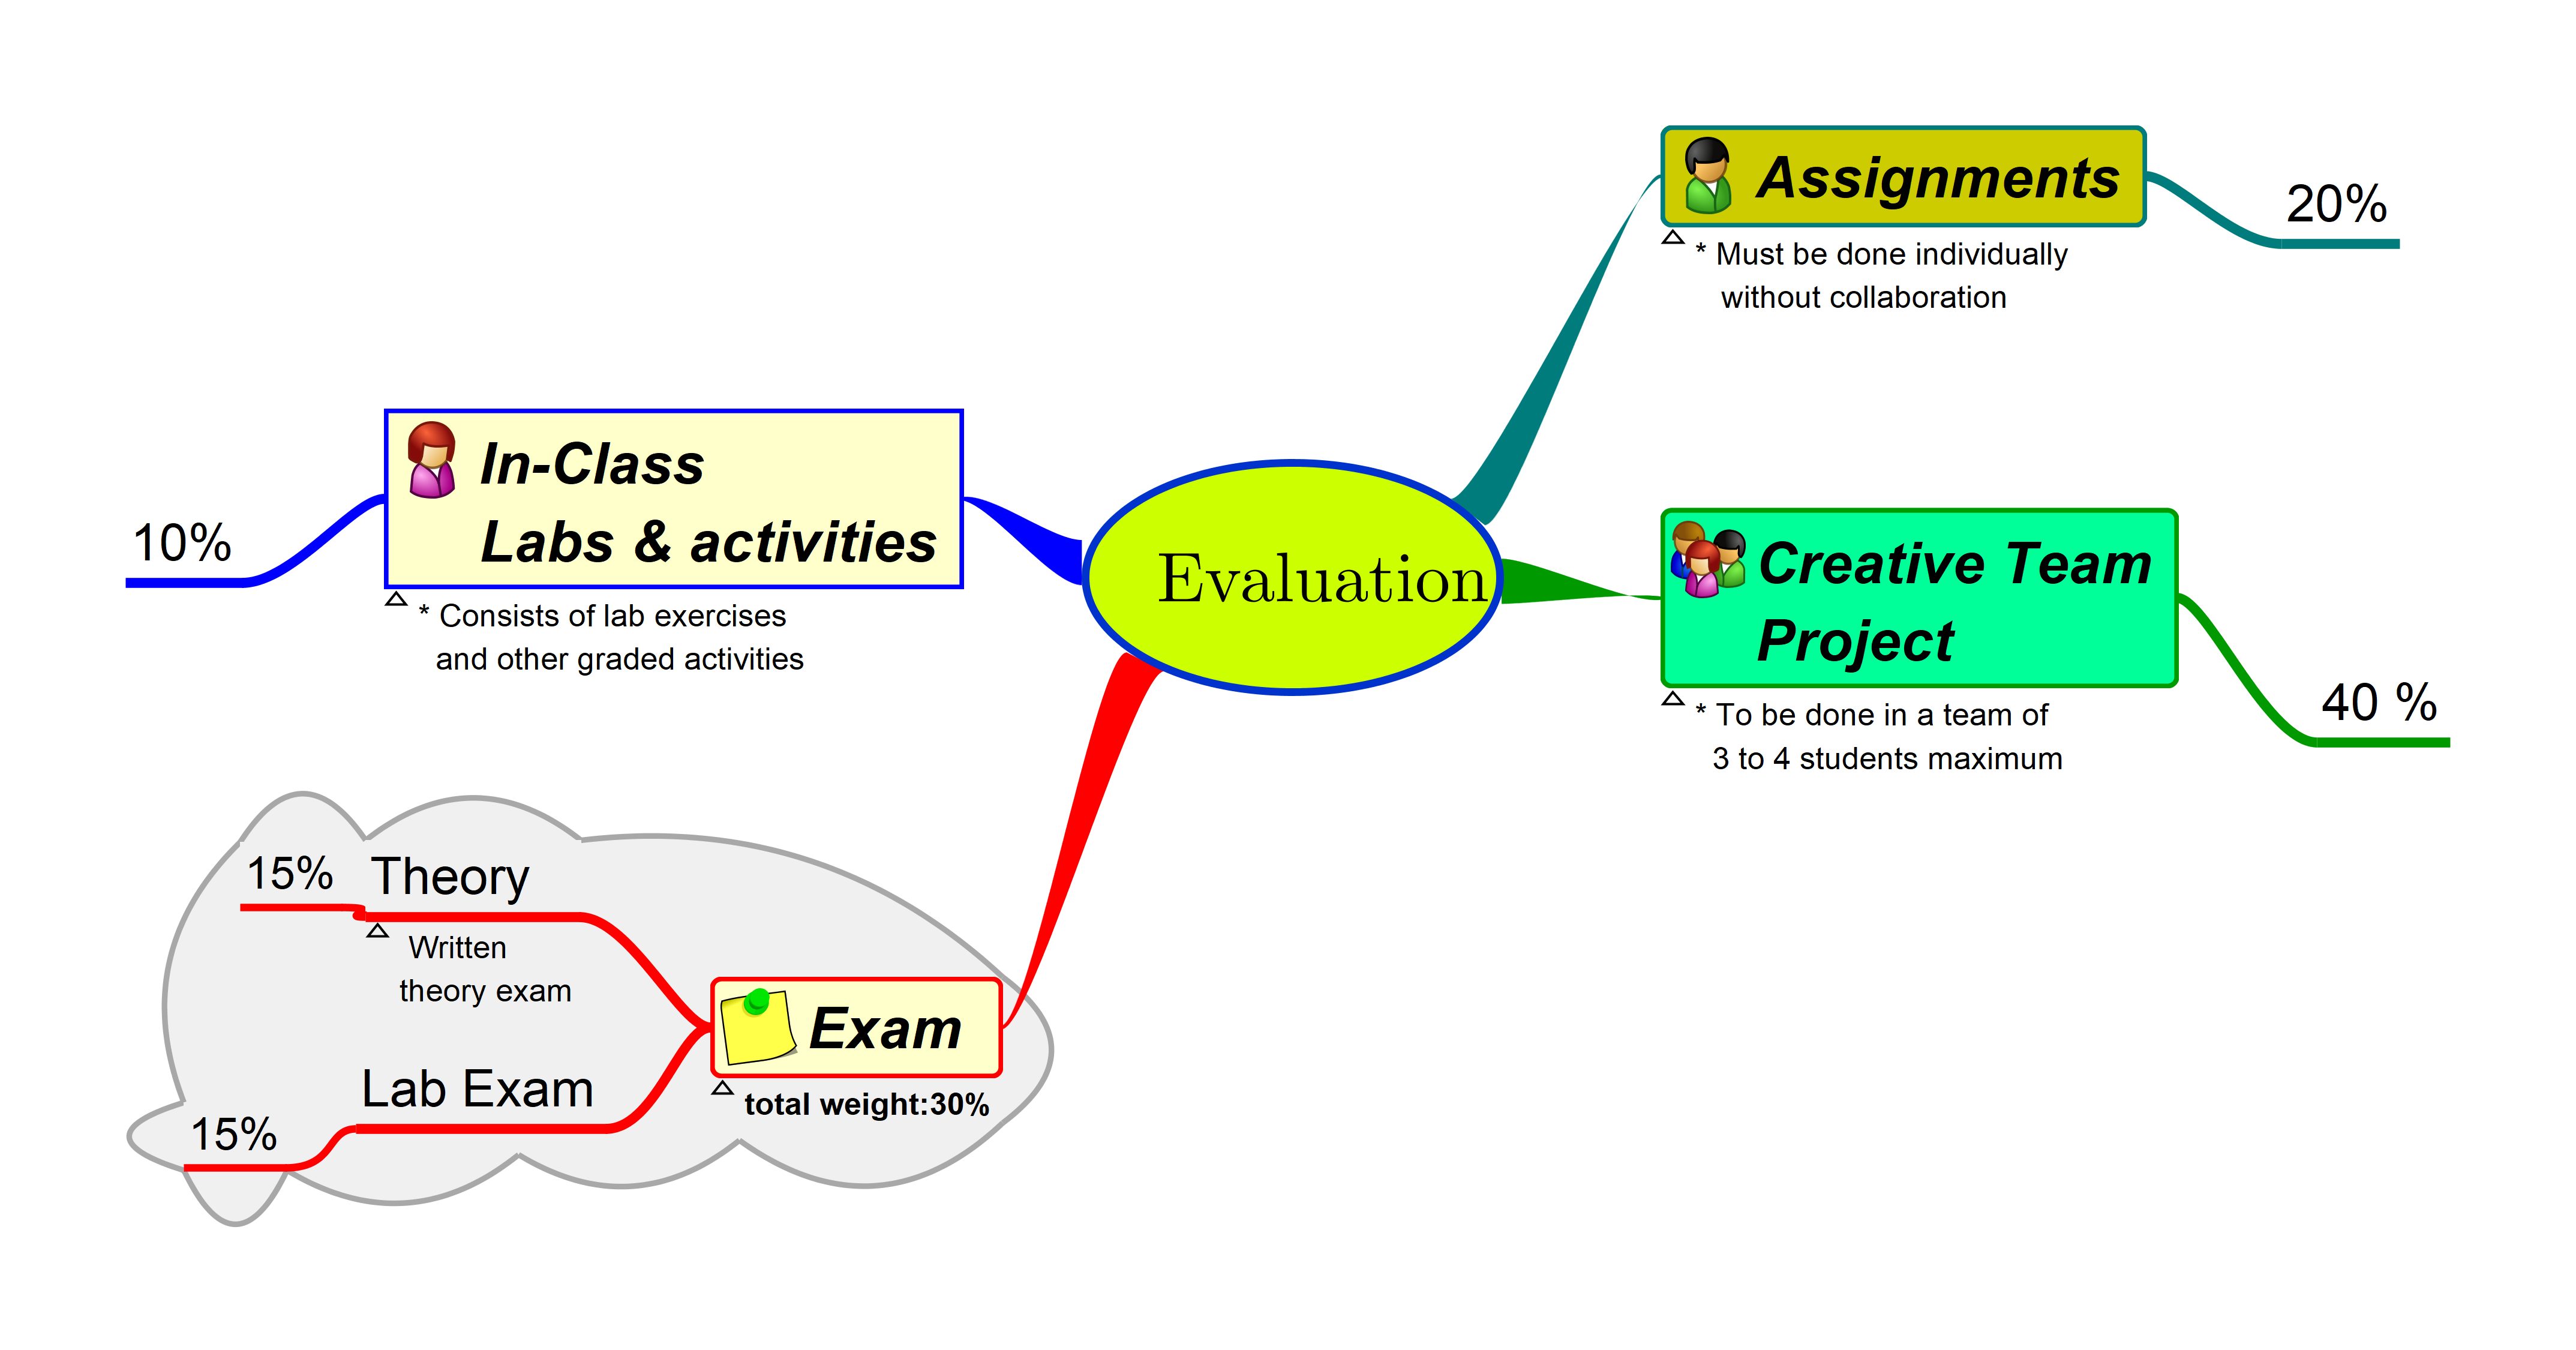
\includegraphics[scale=0.47]{includes/mindmap/A21-Evaluation-420-408.png}
    \vspace{-1.3cm}
    \caption*{
        \small\textit{
            \textbf{\underline{Note:}}
            For a tabular format of this grading scheme, refer to Section \ref{sec:eval-procudures} that is listed in the Appendix below.
        }
    } 
\end{figure}
    
\noindent \textsc{\large\textbf{Notes and Constraints}}
\vspbpara
\begin{arrows}
\item In order to pass the course, students must....
\item Late work is not accepted unless prior arrangement with the teacher...
\item Assignments are demonstrated in-class as part of the marking process to provide feedback before exams. 
\item Students will be informed of the exact date of each test at least one week in advance.
\end{arrows}

\clearpage

\customsection{Textbooks and Course Materials}  
%---------------------------------
%--> List of recommended textbooks. 
\begin{itemize}[itemsep=4pt,parsep=0pt,topsep=1pt,partopsep=1pt]
	\item[\color{darkblue}\faNewspaperO] \textbf{\textsc{Online Resources:}}
	Lecture notes, APIs documentation and online Web tutorials will be provided to students throughout the semester.  \\
	\noindent \textbf{Using Omnivox:} Throughout the semester, students will use Omnivox to download material, upload deliverable files, and obtain all course information.
		
	\item[\color{darkblue}\faBook] \textbf{\textsc{textbook:}} There is no required textbook for this course. However, the following is a list of textbooks that are strongly recommended for this course:\\
\end{itemize}

\hrule
\vspace{.2cm}
\begin{minipage}[b]{0.17\linewidth}          
	
\includegraphics[width=.95\linewidth]{includes/images/unity-in.action.jpg}
\end{minipage}\hfill
\begin{minipage}[b]{0.75\linewidth}          
	\noindent \textbf{Title:} Unity in Action: Multiplatform game development in C\#, 2nd Edition \\
	\textbf{Author:} Joseph Hocking \\
	\textbf{Publisher:} Manning Publications, publication year: 2018  \\
	\textbf{ISBN-13:} 978-1617294969\\         
	\textbf{Available at:}     \href{https://www.manning.com/books/unity-in-action-second-edition}{Manning Publications},
	\href{https://www.amazon.ca/Unity-Action-Multiplatform-game-development/dp/1617294969}{Amazon}
	 and other vendors. 
	 \\
\end{minipage}
\vspace{.18cm}
\hrule
\vspace{.1cm}
\begin{minipage}[b]{0.17\linewidth}          
	
\includegraphics[width=.95\linewidth]{includes/images/UnityCookbook.jpg}
\end{minipage}\hfill
\begin{minipage}[b]{0.75\linewidth}          
	\noindent \textbf{Title:} C\# Game Programming Cookbook for Unity 3D, 2nd Edition \\
	\textbf{Author:} Jeff W. Murray \\
	\textbf{Publisher:} CRC Press; publication year: 2021  \\
	\textbf{ISBN-13:} 978-0367321642\\         
	\textbf{Available at:}     
	\href{https://www.amazon.ca/dp/0367321645/}{Amazon},
	and other vendors. \\
\end{minipage}
\\
\hrule
\vspace{.1cm}
\begin{minipage}[b]{0.17\linewidth}          
	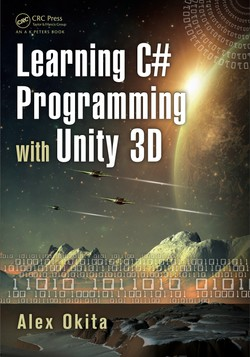
\includegraphics[width=.95\linewidth]{includes/images/learningUnityCSharp.jpg}
\end{minipage}\hfill
\begin{minipage}[b]{0.75\linewidth}          
	\noindent \textbf{Title:} Learning C\# Programming with Unity 3D, 1st Edition \\
	\textbf{Author:} Alex Okita \\
	\textbf{Publisher:} A K Peters/CRC Press; publication year: 2014  \\
	\textbf{ISBN-13:} 978-1498760201\\         
	\textbf{Available at:}     
	\href{https://www.amazon.ca/Learning-C-Programming-Unity-3D/dp/1466586524/}{Amazon},
	and other vendors. \\
\end{minipage}

%--------  Required Software and Material ------------------------------
\vspace{.4cm}

\customsection{Required Software and Tools }  
\begin{itemize}[itemsep=2pt,parsep=0pt,topsep=2pt,partopsep=2pt]
	%    \item[\color{darkblue}\faCoffee] Java 7 or 8 (32 or 64 bits)
	\item[\color{darkblue}\faLaptopCode] \textbf{Operating system:} \faWindows {} Windows  10,  \faLinux {} Linux, \textcolor{vanierred}{\textbf{or}} \faApple {} macOS 
	\item[\color{darkblue}\faCode] \textbf{IDE \& Game Engine:} \faUnity Unity \textcolor{vanierred}{2020.3 (LTS)} \textcolor{darkblue}{\&} Visual Studio \textcolor{vanierred}{2019} (Community Edition)
	\item [{\color{darkblue}\faChrome}] \textbf{Web Browser:} Google Chrome.   
	\item[{\color{darkblue} \faWpforms}] Markdown for writing documentation.
	\item[{\color{darkblue} \faGitSquare}] Distributed version control system.
	\item[{\color{darkblue} \faBitbucket}] Bitbucket: a web-based version control repository hosting service.
	\item[{\color{darkblue} \faTrello}] Trello: a Web-based project management system.
	
	\item[\color{darkblue}\faUsb]
	A storage medium (a USB flash memory or any online free storage service such as GDrive or OneDrive) for storing and backing up your files. 
	\item[\color{darkblue}\faInfoCircle]
	If you want to work at home on your assignments, students must install and use the \textbf{same versions} of the required software that are installed in our labs. \\
\end{itemize}   



 \clearpage
\noindent {\color{darkred} \bfseries\Large\scshape Course Policies} 
\customsection{Class Policy and Rules of Conduct} 
\begin{itemize}[itemsep=2.5pt,parsep=0pt,topsep=8pt,partopsep=4pt]
	\item[{ \color{darkblue} \faLaptop}] Laptops are \underline{strictly prohibited} in classroom during the lectures and labs. 
	
	\item[{\huge \color{darkblue} \faMobile}] 
	\textbf{Cell phones strictly prohibited during classes and labs}. Electronic devices must be turned off (\faBellSlashO) and placed in your bags (not on the desk just in front of you). 
	\item[{\large \color{darkblue} \faHeadphones}] 
	\textbf{Headphones} should be removed all the time.            
	\item[{\color{darkblue} \faEdit}] \textbf{During lectures}, students must turn off their monitors and take notes. Using the computer during lectures without authorization is strictly not allowed. 
	\item[{\color{darkblue} \faMicrophoneSlash}] 
	Video or audio recordings and taking photographs are NOT permitted. 
	\item[{\color{darkblue} \faWechat}] 
	Persistent talking, whispering or any disruptive attitude will not be tolerated.
\end{itemize}

\vspace{0.5cm}
\customsection{Appendix }  
\hrule 
\vspbpara 
 
\customsection{Evaluation Procedures}    
\label{sec:eval-procudures}
    \begin{itemize}[itemsep=8pt,parsep=0pt,topsep=3pt,partopsep=4pt]
    \item[]
%    \begin{center}
        \renewcommand{\arraystretch}{1.5} % this reduces the vertical spacing between rows    
        \begin{tabular}{lcl}
            \thead{\color{darkblue} Course Component} & \thead{\color{darkblue} Overall Weight} & \thead{\color{darkblue}Tentative Period} \\ 
            %---s Load the table body: dynamic table content.        
       \hline    
            \textbf{Individual Homework} &   &   \\                         
                   \hline    
		\textit{Assignment}  &  20\% &  Week 2-7 \\                           
         \textit{In-class labs}  &  10\% &  Week 1-11 \\                           
          \hline    
        \textbf{Exam} &   &   \\                         
           \hline
            \textit{Theoretical exam} &  15\% &  Week 7 \\               
            \textit{Lab exam} &  15\% &  Week 8 \\               
            \hline
           \textbf{LIA} &   &   \\                         
		\hline
			\textit{Team project} & 40\% & Week 2 to 15 \\               
        \hline


        \end{tabular}
        \vspace{-1em}
%    \end{center} 
    %        \evaluationrules
\end{itemize}  
\clearpage

\customsection{Tentative Course Content}
%TODO: split implementation into 3 builds.
\renewcommand{\arraystretch}{1.5} % this reduces the vertical spacing between rows    
\noindent\begin{tabular}{|p{1cm}|p{15cm}|}
	\hline
	\thead{\color{darkblue} Week} & \thead{\color{darkblue}Topics \& Homework} \\ 
	\hline
	%---s Load the table body: dynamic table content.        
	\textbf{1} &   Course outline discussion \& team Project Guidelines    \\
	& \labactivities \\
	\hline    
%	 Week 2
	\textbf{2} & Topics... \\
		& \labactivities \\
	& \redtext{\textbf{Announcement:...} Assignment \#1}\\
\hline    
%	 Week 3
	\textbf{3} &  Topics... 
	\\
	& \labactivities { }\redtext{Team project proposal due.}\\ 
\hline
%	 Week 4	
	\textbf{4} & Topics... \\
    & \labactivities { }\redtext{Game Design Document due.}\\
\hline
%	 Week 5	
\textbf{5} & Topics...
\\
& \labactivities { } \redtext{Team project proposal presentations.}\\
\hline
%	 Week 6	
\textbf{6} & Topics...\\
\hline
%	 Week 7	
\textbf{7} & Review for exam. \redtext{Assignment due.}
\\
\hline
%	 Week 8	
\textbf{8} & \textbf{Exam} \& work on team project.
\\

\hline
%	 Week 9
\textbf{9} & Topics...\\
	\hline
%	 Week 10
\textbf{10} & Topics...\\
& \redtext{Build \#1 due.}\\
  \hline
%	 Week 11
\textbf{11} & Topics...\\
& \redtext{TCR Checklist due.} \\
 \hline
 %	 Week 12
\textbf{12} & Topics...\\
& \redtext{Build \#2 due.}\\
 \hline
 %	 Week 13

 \textbf{13} & Work on team project.\\
\hline 
 %	 Week 14
\textbf{14} &  Playtesting session. \\
& \redtext{Build \#3 due.}\\
\hline  
 %	 Week 15
\textbf{15} & Final project demonstrations. Peer review due. \\
& \redtext{QA testing report \& user guide due.}\\
\hline  
\end{tabular}   

\vspace{1cm}
\noindent \textcolor{red}{\textbf{\underline{NOTE:}}} The above actual dates may be modified due to the requirements of the class. Also, the indicated dates may be moved backward or forward depending on class progress. \textbf{Exact dates and instructions will be announced on course webpage}. 

\end{document} 